\documentclass[a4paper]{article}

\usepackage{fullpage} % Package to use full page
\usepackage{parskip} % Package to tweak paragraph skipping
\usepackage{tikz} % Package for drawing
\usepackage{amsmath}
\usepackage{hyperref}

\title{CSCI 33500: Software Analysis and Design III}
\author{Summer 2025}
\date{Midterm Review}

\begin{document}
\maketitle


\section{TRUE OR FALSE}
\begin{enumerate}
    \item little o notation is used to represent an algorithms best case performance
    \item when do you need to write the big 5 ? 
    \item The time complexity of search, insertion, and deletion operations in an AVL tree is O(log n).
    \item An algorithm with time complexity O(n!) is more efficient than one with time complexity O(n log n).
    \item The Big Five in C++ include the default constructor, copy constructor, move constructor, copy assignment operator, and destructor.
    \item The compiler distinguishes between the move constructor and the copy constructor based on whether the argument is an lvalue or an rvalue.
    \item The space complexity of the selection sort algorithm is O(1)
    \item If a function $f(n) \in \Theta(n log n)$, then $f(n) \in O(n log n)$ and $f(n) \in \Omega(n log n)$.
    \item In a proof by induction, the base case is optional as long as the inductive step is valid.
    \item AVL tree insertions may trigger a rotation to maintain the balance condition. 
\end{enumerate}
\newpage


\section{SHORT ANSWER}
\begin{enumerate}
    \item  x = 49 mod 9. assume x is greater than or equal to 0 and less than 9, what is x ?  
    \item solve gcd(318, 1002)
    \item Which proof technique would you use for for the following question:\\ show that \[ \sum_{k=0}^{n} x^k = \frac{x^{n+1}-1}{x-1}\]    
    \item Write the code for an ll rotation in an avl tree. 
    \item is the following function declaration correct? \begin{verbatim}
        bool my_func(int val1=12,int val2);
    \end{verbatim}
    \item Give the summation series for: 15, 21, 27, 33, ..., 177
    \item Simplify the following function using big O notation. $3\frac{n}{7} +log(n) +3m +1000000$
    \item Given the following code, what will be printed ?\\ 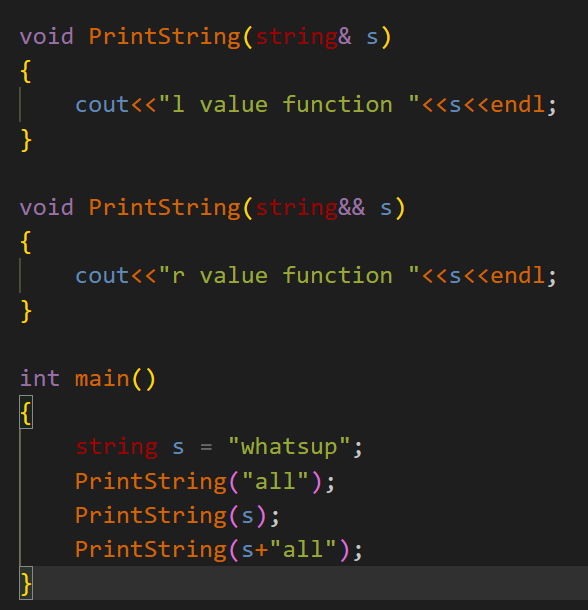
\includegraphics[width=0.5\textwidth]{exam_question.png} 
    \item prove the following, if x is even then $x^2$ is also even. 
    \item what does std::move do ?
\end{enumerate}
\newpage 


\section{CODING}
\begin{enumerate}
    \item Write a recurrence relation for the power set(the power set is the set of all subsets for a given set), then compute the big O from your recurrence relation. 
    Using vectors write the code to print the power set for any given set of size 3, what is the big O, big $\Omega$ and Big $\Theta$  for the code you wrote? 
    
    \item Given selection sort do an average time complexity analysis.
    \begin{verbatim}
    void selection_sort(int* arr, int size)
    {
        for(int i=size-1;i>0;i++)
        {
            int max_index=0;
            for(intj=1;j<=i;j++)
                if(arr[j]>arr[max_index]) max_index=j;
            std::swap(arr[i],arr[max_index]);
        }
    }
    \end{verbatim}
\end{enumerate}
\end{document}